%! Author = felix
%! Date = 17/03/2024

\renewcommand{\kapitelautor}{Autor: Felix Zwickelstorfer}
\subsection{Parser}\label{subsec:parser}
\renewcommand{\kapitelautor}{Autor: Felix Zwickelstorfer}

Der Parser nimmt einen Text in "raw" und zusätzlich eine Liste an Objekten, welche Beschreiben, wie dieser Text am Ende aussehen sollen beziehungsweise welche Besonderheiten vorkommen.
Dabei wird aus jedem vollständigen Wort (von einem Leerzeichen oder einem Zeilenumbruch getrennt) zu einem eigenen Element, was es erlaubt, dass man den Text in verschieden Weisen hervorheben kann.
Dies ermöglicht es, dass diese Elemente einen dynamischen Zeilenumbruch haben, falls sich die Werte innerhalb verändern.
Weiteres gibt es die Möglichkeit diverse Icons in den Text einzubinden.
Zusätzlich kann man den Text in anderen Weisen hervorheben als nur Schriftart und Größe durch \zB das Bewegen des Textes.

Dies kann man beispielsweise am Hovertext von der Bullet Bullet erkennen:
\begin{figure}[H]
    \centering
    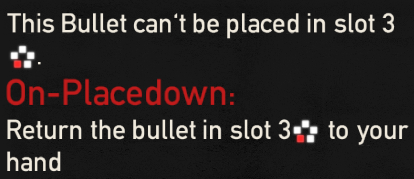
\includegraphics[width=0.7\textwidth]{hovertext_bulletbullet.png}
    \caption{Screenshot des Hovertexts der Bullet Bullet}
\end{figure}


%TODO Zwicki
% Savestates 0.5 Seiten
%   wenn perma gelöscht, kompletter reset, auch mit user prefs
% key input 1 Seite
% road generation 3 Seiten
% Shop, ChooseCard hinzufügen 1 Seite
% Inputfeld 2 Seiten